% This gives a good opportunity to briefly describe the data architecture of your company
% You must show you have considered all relevant data protection policies and regulations (both internal company policy and external laws or guidelines).
% If you use any data external to the company you must reference it.
% Justify the choice of the data and why it is relevant to the project
% State what tools you used to efficiently gather the data
% Outline briefly the data cleansing steps you have taken and the consideration of any source of error and bias

\section{Data selection, collection and pre-processing}

% Data architecture

A programme of the BBC iPlayer catalogue is mapped internally by a hierarchy of items defined by an ID called \textit{PID}.
An item can be of type \textit{episode}, \textit{series}, or \textit{brand}. The \textit{episode} is the leaf of this tree-like structure,
representing the playable content like an episode of a series, a live show, or a one-off, like a movie or documentary.
In contrast, \textit{series} and \textit{brand} types are considered ``containers'' and appear at the upper levels of the tree.
Their children can be other containers or \textit{episode} items \cite{BBC:ProgrammePages,BBC:ProgrammeUrlStructure},
[figure \ref{fig:program_hierarchy}] and [figures \ref{fig:pips_brand}, \ref{fig:pips_series}, \ref{fig:pips_brand_series} of the appendix].

\begin{figure}[h]
  \centering
  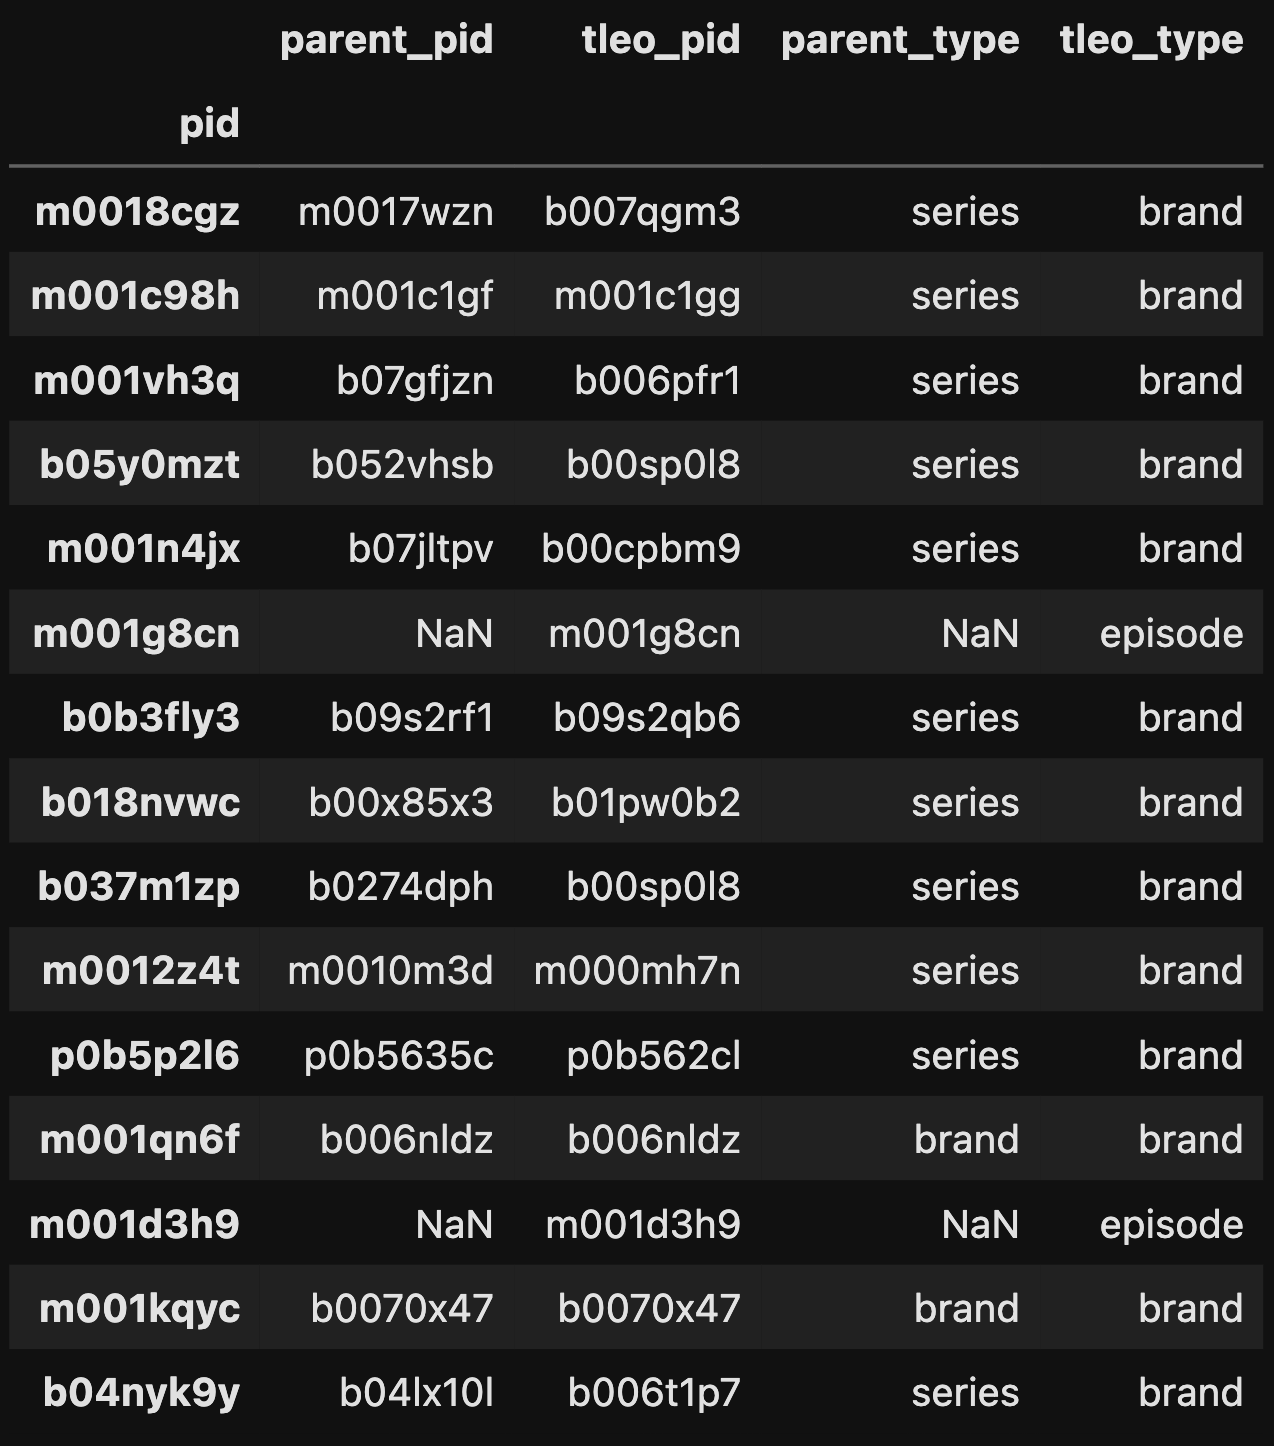
\includegraphics[scale=0.2]{program_hierarchy}
  \caption{Internal programme hierarchy structure}
  \label{fig:program_hierarchy}
\end{figure}

Each item of this tree-like structure represents a part of the programme
(a single episode, a season, or the programme itself)
and shares the same Passport tags by inheritance.
These items are the dataset's rows, replicating the same set of tags for any given programme.
This duplication was used as a data augmentation training technique to increase the model's performance.

BBC News and Sport articles, iPlayer videos, and Sounds audios are annotated with Passport tags.
These tags describe any BBC content and can be used for retrieval (search) and filtering (recommendations).
They can be applied manually by an editorial team with domain knowledge
or semi-automatically by machine learning algorithms with human supervision.

Passport tags are distributed across the BBC via the universal content exposure and delivery (UCED) system.
This self-service delivery platform exposes data as a document stream for products to integrate.
It provides different types of consumers, such as REST API, AWS S3 bucket, etc.
Passport documents are JSON objects that contain a property called ``\verb|taggings|'', an array of objects representing the
metadata annotations. Two properties describe these objects: ``\verb|predicate|'' and ``\verb|value|''.
They represent a tag's name and value and are expressed as URL-formatted strings, except for dates [figure \ref{fig:passport_file}].

\begin{figure}[h]
  \centering
  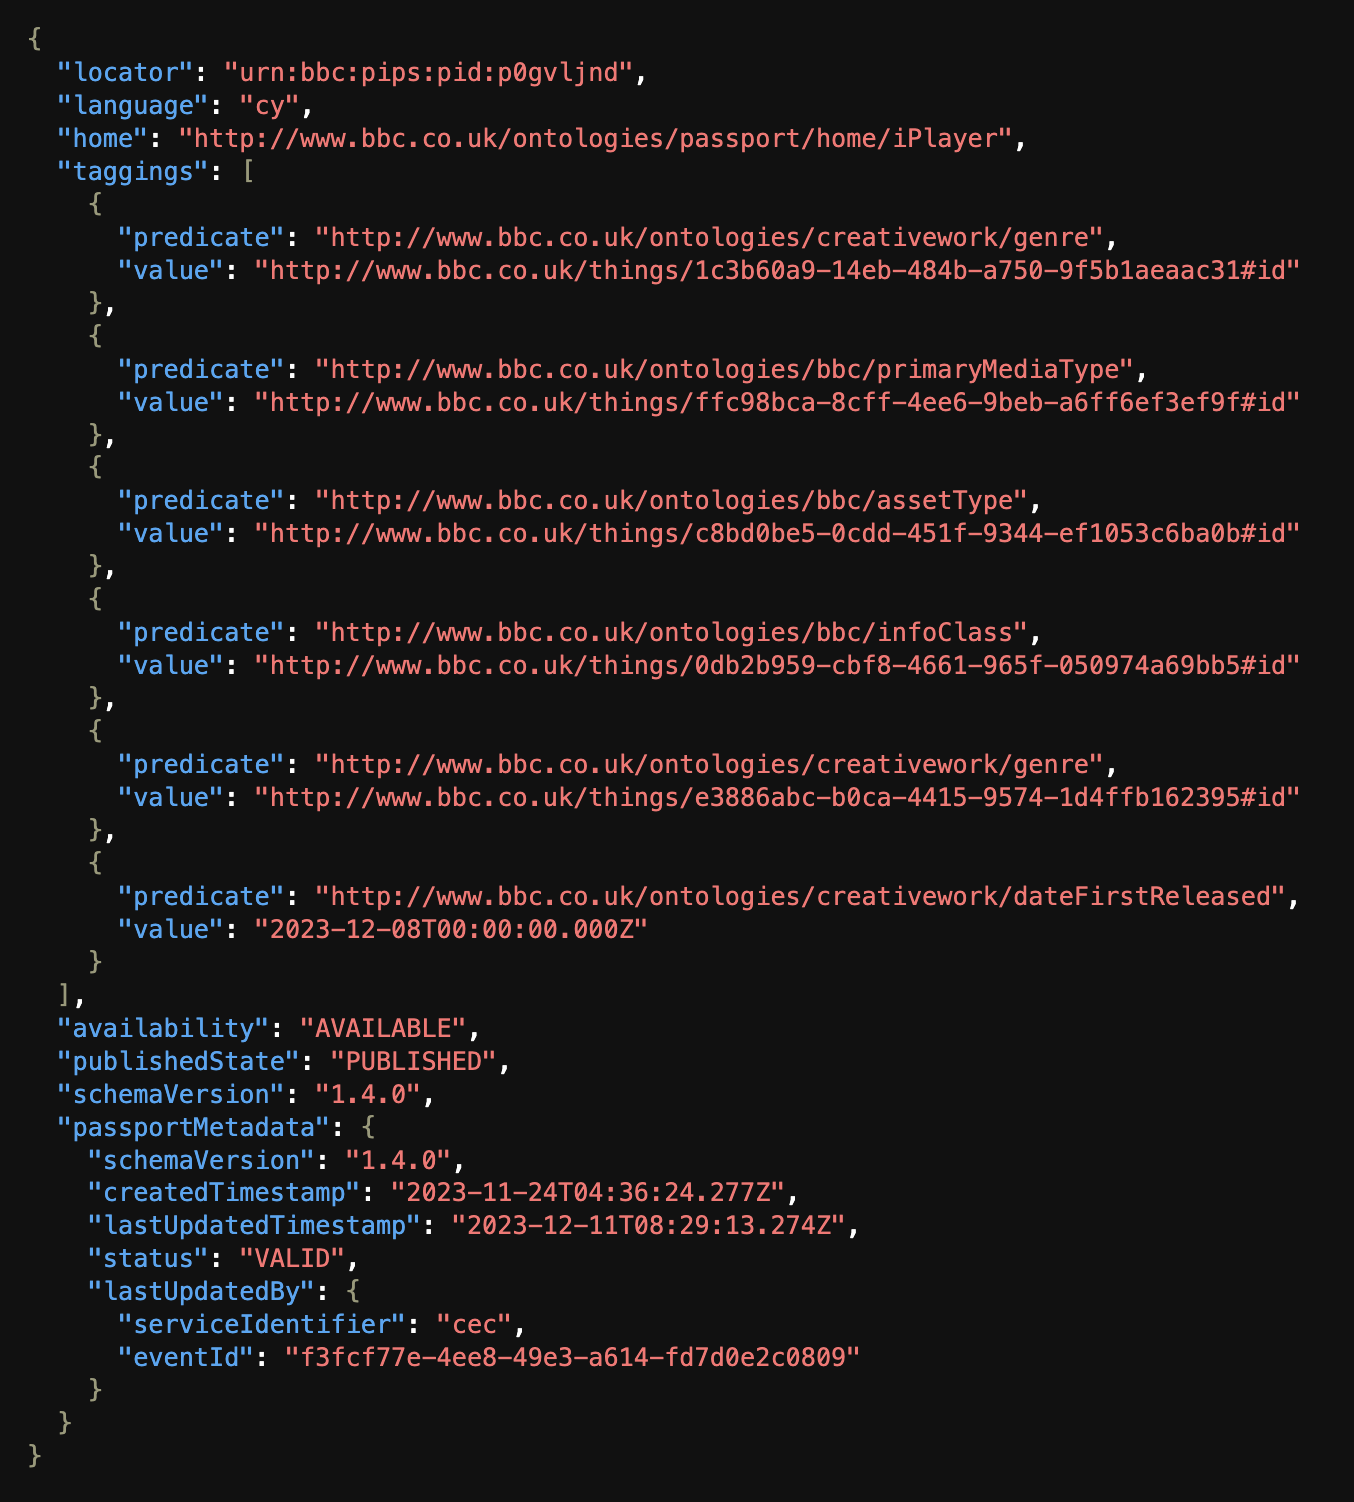
\includegraphics[scale=0.3]{passport_file}
  \caption{An example of Passport file}
  \label{fig:passport_file}
\end{figure}

The predicate is a class of the BBC Ontologies \cite{BBC:Ontologies} and describes the annotation.
The value can be a date or a BBC Things entity \cite{BBC:Things,BBC:Things:About} defined as an RDF document \cite{W3C:RDF,W3C:RDF:Concepts},
described by other BBC Ontology classes and accessible in Turtle format \cite{W3C:Turtle} via the BBC Things API \cite{BBC:Things:API}.
These entities are linked to each other and other external resources and form a graph data structure.

% Tools used to gather data

I decided not to integrate with UCED during development but to use batches of Passport files,
manually collected and stored in a local folder.
This trade-off allowed me to train the model with live data while reducing costs.
In addition, because I had to create resources on two AWS accounts,
I did not want to pass the burden of maintenance to the team that owned them without having tested the feasibility of the solution first.

% Data protection policies and regulation

Content metadata does not constitute personal data and, therefore, is not subject to the UK GDPR  \cite{UKGDPR}.
Nonetheless, this data is encrypted at rest and in transit by default.
For this reason, no further actions were required during storage and processing.

% Data choice justification and relevance

I chose to use Passport because it provides a set of tags shared across all BBC content,
making this a general solution that reduces duplications and costs.
Passport offers a flexible and rich set of tags to describe any type of content.
The eight annotations I selected for training were:
\verb|about|, \verb|genre|, \verb|format|, \verb|contributor|, \verb|motivation|,
\verb|editorialTone|, \verb|narrativeTheme| and \verb|relevantTo|
(see figures \ref{fig:passport_stats}, \ref{fig:tag_about}, \ref{fig:tag_contributor},
\ref{fig:tag_editorialTone}, \ref{fig:tag_format}, \ref{fig:tag_genre}, \ref{fig:tag_motivation}
\ref{fig:tag_narrativeTheme} and \ref{fig:tag_relevantTo} for example values).

% Data preprocessing, errors, bias

The dataset used for training contained all the programmes available in the iPlayer catalogue from \verb|13 June 2023| to \verb|15 April 2024|.
The catalogue had \verb|83098| items, \verb|81311| of which were annotated with Passport tags stored in JSON files, amounting to a coverage of \verb|97.85%|.
The pipeline's pre-processing stage loaded these files [figure \ref{fig:passport_file}] into a dictionary data structure [code \ref{lst:data_loading}].
The dictionary's key was the \textit{PID} and the value was another dictionary describing the annotations [figure \ref{fig:dataset}].

\begin{figure}[h]
  \centering
  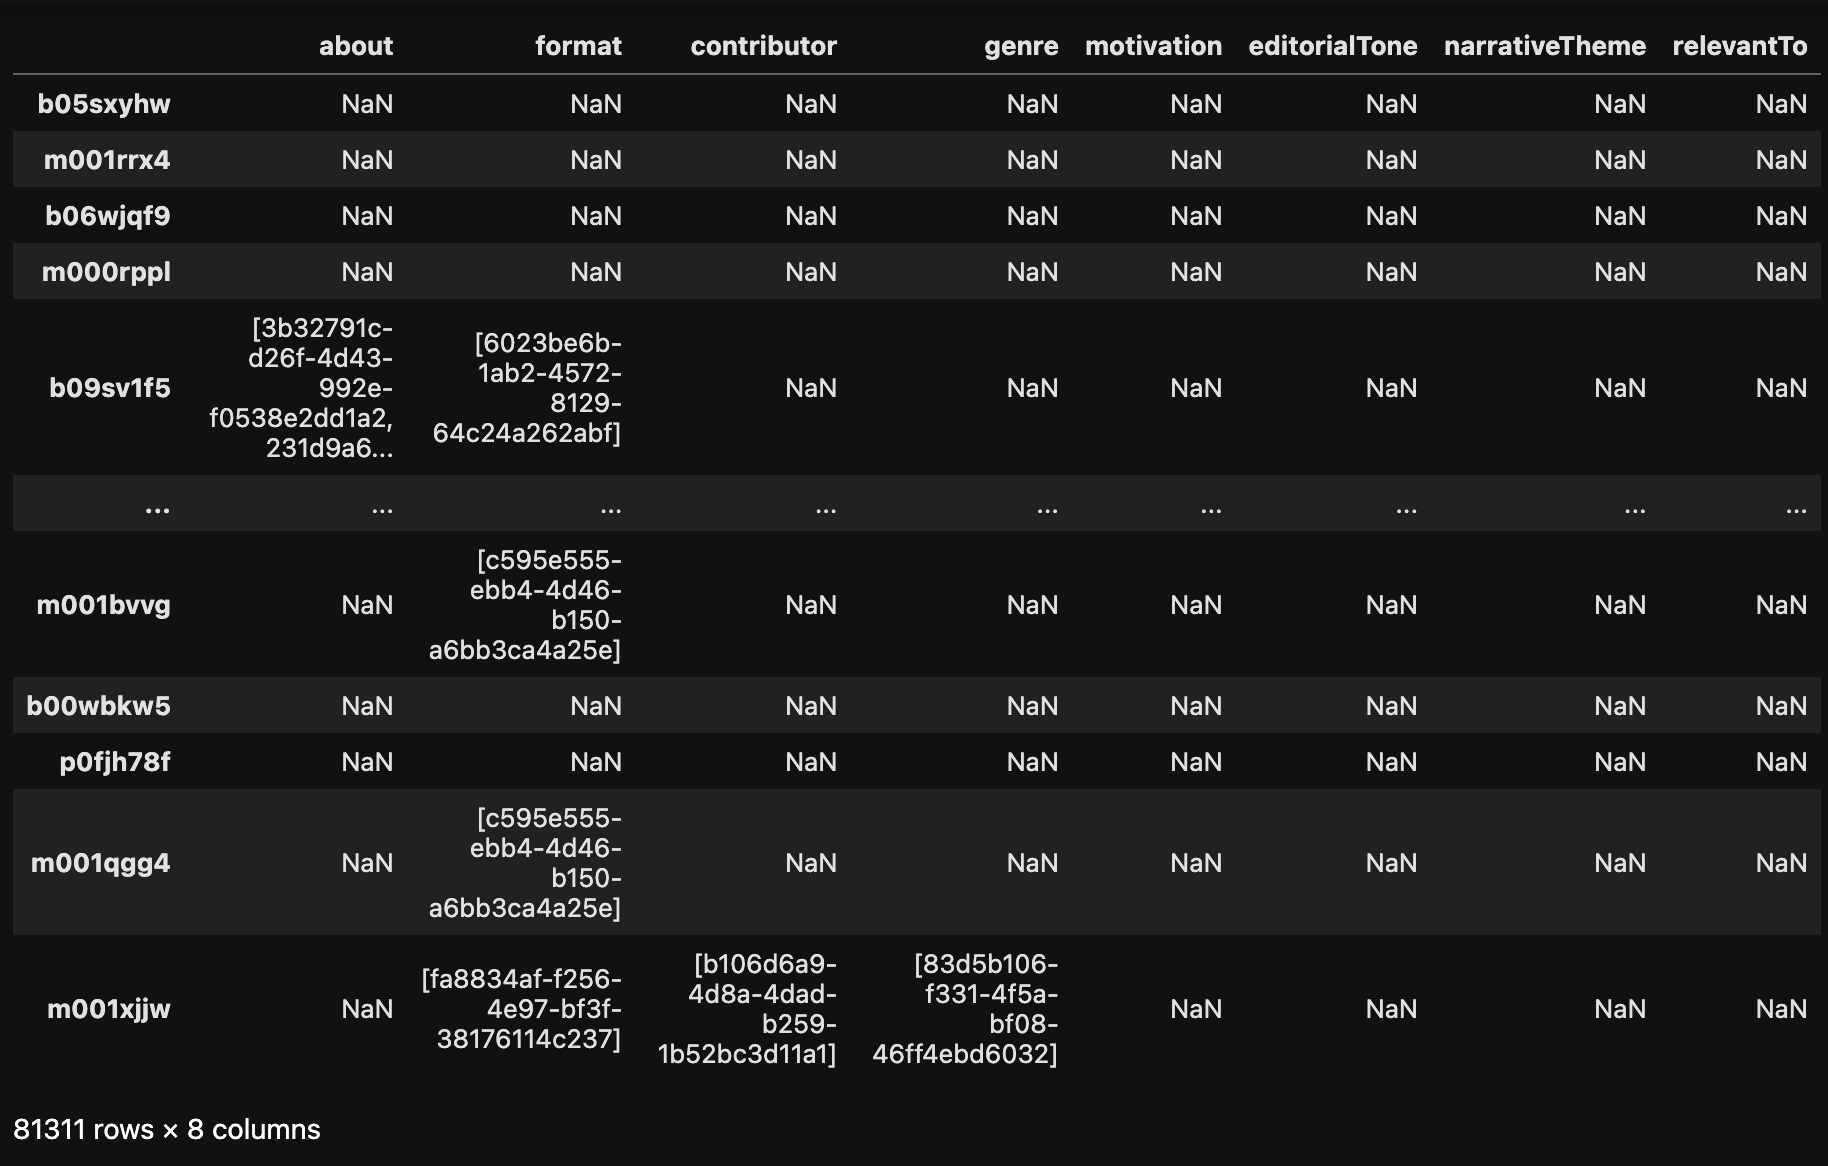
\includegraphics[scale=0.3]{dataset}
  \caption{A DataFrame visualisation of the dictionary data structure}
  \label{fig:dataset}
\end{figure}

A programme can be tagged with the same predicate multiple times [figure \ref{fig:dataset_row}] if it has different values,
while the same value (e.g. ``Music'') can be used by various predicates (e.g. \verb|about| or \verb|genre|).

\begin{figure}[h]
  \centering
  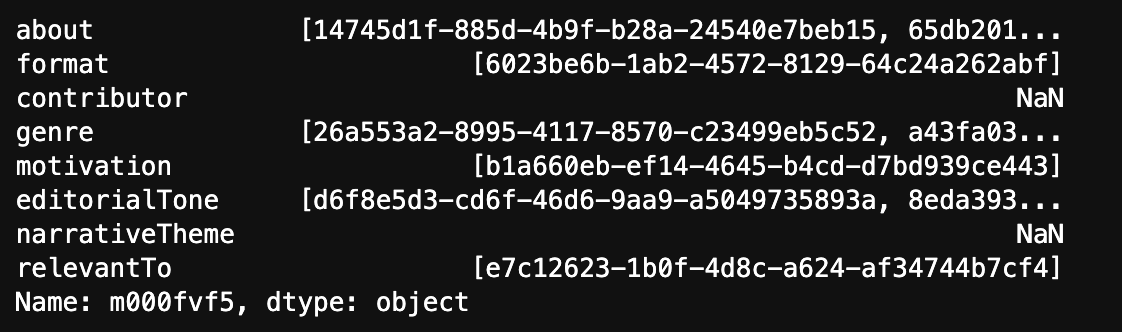
\includegraphics[scale=0.5]{dataset_row}
  \caption{A sample programme with tagging}
  \label{fig:dataset_row}
\end{figure}

The pipeline then created a Pandas \textit{Dataframe} pre-populated with zeros,
where the rows represented the programmes, and the columns represented the tags.
I used a MultiIndex \cite{Pandas:MultiIndex} for the columns because it needed to keep track of the duplicate values (2nd-level index)
across the predicates (1st-level index) to access the cells to populate them with the value ``\verb|1|''
if the programme was annotated with the corresponding tag, generating one-hot encoded arrays [figure \ref{fig:dataset_encoded}] [code \ref{lst:data_encoding}].

\begin{figure}[h]
  \centering
  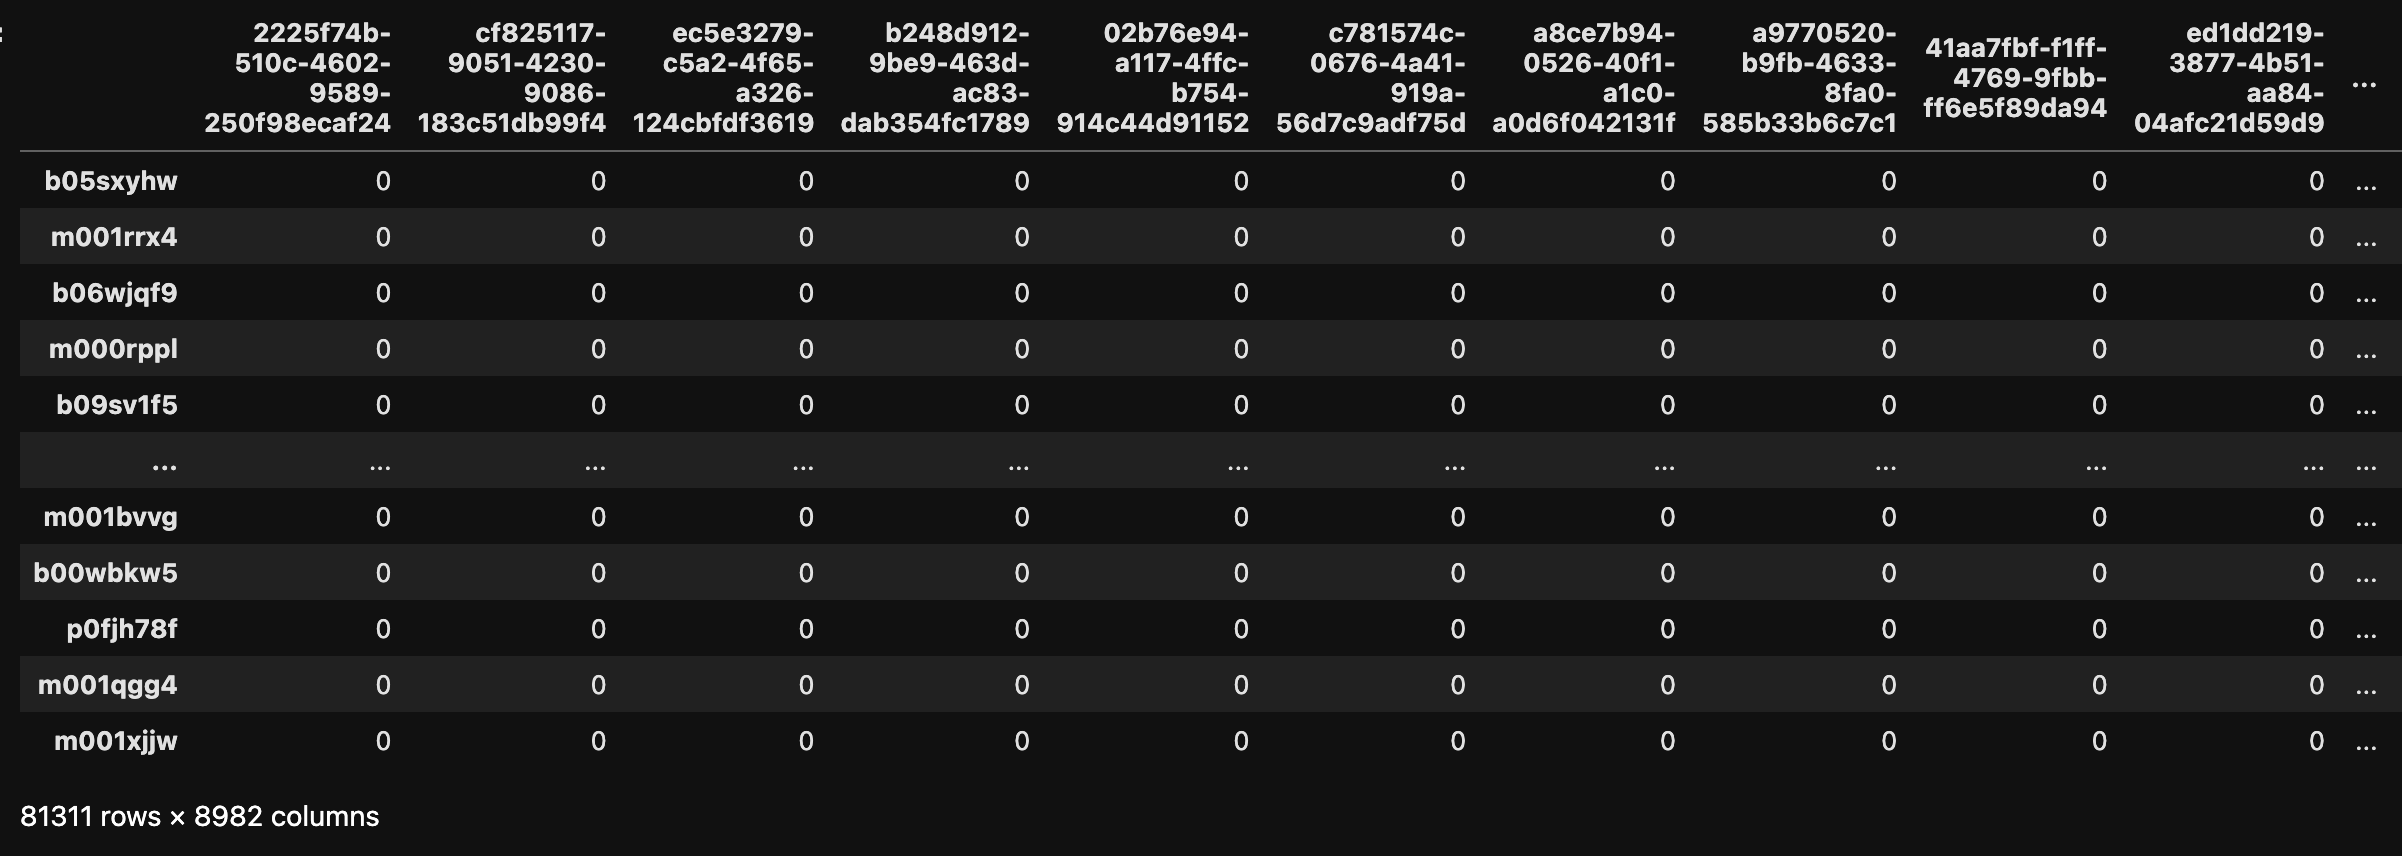
\includegraphics[scale=0.3]{dataset_encoded}
  \caption{The one-hot encoded dataset}
  \label{fig:dataset_encoded}
\end{figure}

One-hot encoding is positional and does not care about the actual tag labels,
so I decided to extrapolate the URL identifiers [figure \ref{fig:dataset_column}] and use them as tag values,
speeding up the data loading stage because it did not need to fetch the labels from the BBC Ontology.

\begin{figure}[h]
  \centering
  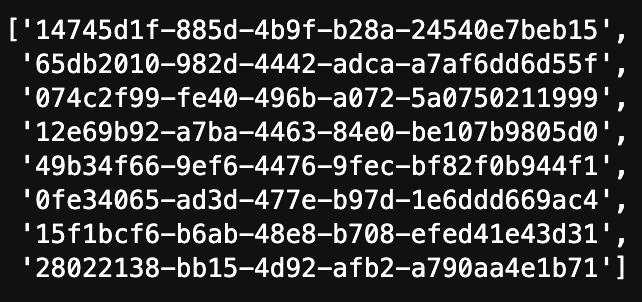
\includegraphics[scale=0.5]{dataset_column}
  \caption{A list of hashed values for a given tag}
  \label{fig:dataset_column}
\end{figure}

A source of bias in the dataset was the \verb|mentions| tag.
This annotation type is automatically generated by an algorithm that extracts terms deemed important,
appearing in the text of an article or the transcript of an audio/video content.
If something is mentioned, it does not necessarily describe the content because of the intrinsic ambiguities of natural languages.
Figure of speech devices, such as metaphors, analogies, allegories, and others, alter the meaning of a sentence for stylistic effect
and can misrepresent the main topic.
For example, if the phrase ``being over the moon'' is mentioned by someone delighted about something unrelated to the topic of ``space'' and ``universe'',
extracting the term ``moon'' as a descriptor could mislead the representation.
To mitigate this source of bias, I dropped \verb|mentions| in favour of \verb|about|,
a tag that describes the main topics of the programme, annotated by a team of editorials with domain knowledge,
trained in unconscious bias management and how to use relevant tags for a given programme.

Generating embeddings of one-hot encoded vectors with the same size used in training but with
unseen tags leads to unpredictable errors.
The encoding is positional, and the combination of \verb|1| and \verb|0| learned by the model
belongs to the tags seen during training. So, I decided to drop the new tags and encode only the ones the model was trained on
while padding the rest with zeros, pending retraining to capture the new information.
Also, some programmes did not have any annotations entirely. Adding them to the training data, created a group of entries with all zeros.
If enough observations shared this uninformative characteristic, the model could have picked it up.
I decided to drop these programmes and include only the ones with at least one annotation.
